%!TEX root = ../main.tex

\section{Aim of the experiment}
The low temperature properties of different solids are determined in the experiment. Especially the electrical resistance of metals, semiconductors and superconductors. We expect a phase shift for the superconductor which requires special consideration. 

\section{Electrical resistance of metals}


A simple description with the Drude model can be used for metals. The electrons are accelerated in an electric field and scattered at the atomic cores after a mean free path. It follows for the electrical conductivity:
\begin{equation}
    \sigma = \frac{ne^2\tau}{m_e}
\end{equation}
where n is the charge carrier density, $\tau$ is the mean free time, and e is the elementary charge. The temperature dependent conductivity follows from the mean free time $\tau$. This is due to the scattering of electrons by phonons and impurities in the lattice. The resistivity is given by $\sigma =\frac{1}{\rho}$ to Matthiessen's rule:
\begin{equation}
    \rho = \rho_{ph}(T) + \rho_{im}
\end{equation}
The scattering at impurities is independent of temperature and is reflected in a constant residual resistance. The following temperature dependencies apply to phonon scattering:
\begin{itemize}
    \item For high temperatures ( $T > \Theta_D$, with $\Theta_D$ Debye temperature).
    \begin{equation}
        \rho_{ph} \propto T
    \end{equation}
   \item For low temperatures ($T<\Theta_D$) 
    \begin{equation}
        \rho_{ph} \propto T^5
    \end{equation}
    
\end{itemize}
Where for high temperatures, according to Grüneisen-Bornelius, one can determine the Debye temperature with:
\begin{equation}
    R_T = 1,17\frac{R(\Theta_D)}{\Theta_D} T-0,17\cdot R(\Theta_D)
\end{equation}


\section{Semiconductors}
Semiconductors are very different from normal conductors like metals. For $T \rightarrow 0$ the valence band is completely filled and the conduction band is empty. One can distinguish between intrinsic and extrinsic semiconductors.


\subsection{Intrinsic semiconductor}


Since neither a full valence band nor an empty conduction band contributes to charge transport, the electrons have to overcome an energy gap $E_{gap}$ to the next band. This is done by thermal excitation, which is obviously temperature dependent. Thus for the electrical conductivity follows:
\begin{equation}
    \sigma_{tot} = \sigma_e+\sigma_h =n_ie(\mu_e+\mu_h)
\end{equation}
where $n_i$ corresponds to the electron / hole density and $\mu$ to the corresponding mobility. In the end, the following equation is obtained:
\begin{equation}
    \sigma_i = C_i \exp{\left (-\frac{E_{gap}}{2k_BT}\right)}
\end{equation}
Thus, the electrical conductivity approaches the constant $C_i$ asymptotically.


\subsection{Extrinsic semiconductor}
By doping a semiconductor, its conductivity can be strongly increased. In this process impurities of the neighboring main group are added. These atoms either donate electrons (donors) or accept electrons (acceptors) and produce a n/p doped semiconductor. Sub-energy levels are created in the band gap which can be excited more easily. This results in a complicated temperature profile with $\sigma = en\mu$.
\begin{figure}
    \centering
    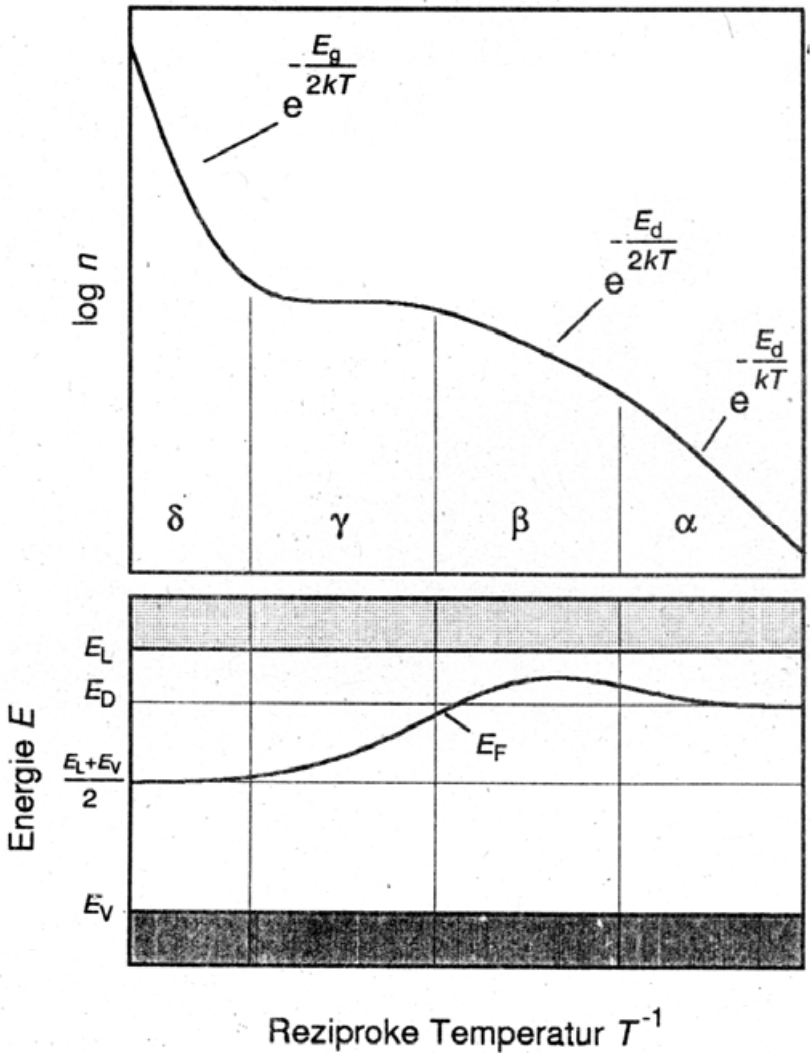
\includegraphics[width=0.5\textwidth]{./fig/exhl.png}
    \caption{Temperature dependent charge carrier concentration in extrinsic semiconductors.}
    \label{fig:exhl}
\end{figure}


\section{Superconductors}

\section{Experimental setup}
